\section{Proposed Method}
\begin{figure*}[t]
    \centering
    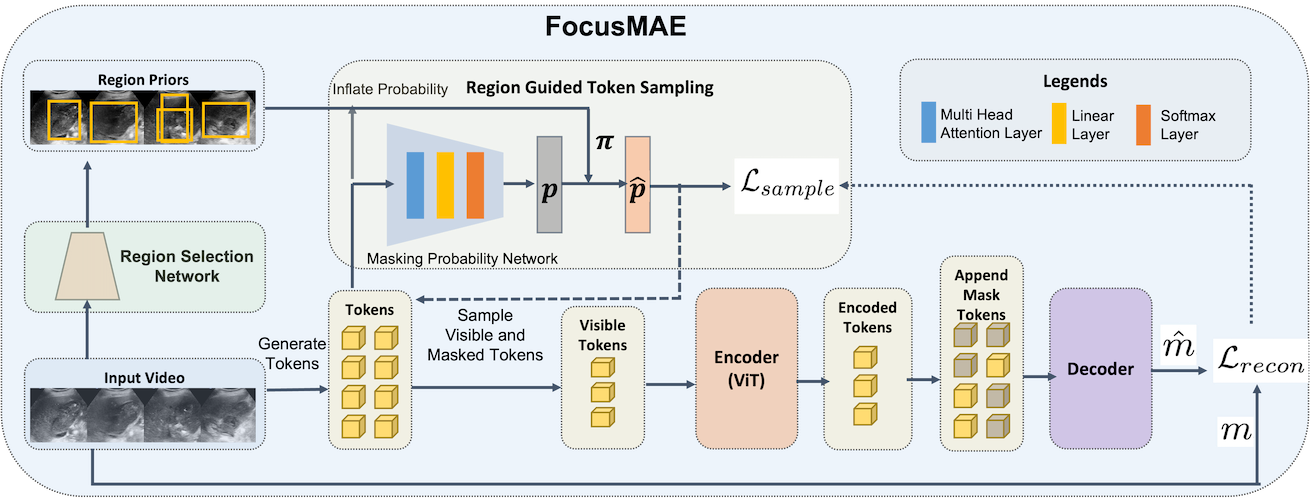
\includegraphics[width=\textwidth]{figs/focusmae/arch.png}
    \caption[Overview of the FocusMAE pipeline]{Overview of the FocusMAE pipeline. Our design proposes guiding the masking tokens with the localization of the candidate focus regions containing high-information. The systematic biasing with focused high-information region priors helps to build a more meaningful reconstruction task for disease representation learning. }
    \label{focusmae_fig:arch}
\end{figure*}

\subsection{Object Priors in MAE}
%
Visual data often demonstrate sparser semantically meaningful information distribution dominated by the foreground objects. Current MAE techniques predominantly use random masking, which may result in sub-optimal performance as the information may not be uniformly distributed. For the USG videos, GBC often occupies a very small portion of the frames. Random masking mostly biases the networks to learn representations of redundant backgrounds containing other organs or abdominal cavities. To alleviate the issue, %we advocate exploiting the object location priors with high information density to enhance the representation learning in MAE. 
we advocate leveraging the object localization priors characterized by high information density to enhance the representation learning in MAE.
We show in \cref{focusmae_fig:teaser_b} the preliminary evidence of potential advantages of boosting the masking token probability with object localization priors. We selected a random validation split containing about 20\% of our GB USG Video dataset. We used the malignant ROI boxes provided in the dataset to specify object locations. We manually increased the masking probability of patches within the bounding box region for the data samples, and used them for self-supervised pretraining. We varied the probability boosting values, denoted by $\pi$, representing the increased probability for patches within the bounding box region as compared to the patches from the background. Our experiment reveals that elevating the probability of masking for patches from the bounding box region, as opposed to random masking, leads to a noticeable enhancement in results. %However, highly inflating the masking probability for patches from the bounding box region may compromise the integrity of the pretext task and result in performance degradation. 
However, excessively inflating the masking probability for patches from the bounding box region may compromise the integrity of the pretext task and consequently lead to performance degradation.
These findings underscore the importance of recognizing that distinct image patches contribute differently to the learning of visual representations. Furthermore, the emphasis on reconstructing foreground objects with a balanced approach is crucial for optimal performance.

\subsection{\focusmae Architecture}
%
\label{sec:method_subsample}
\mypara{Video Sub-sampling}
% 
Video data contains temporal redundancy as the consecutive frames see a very high overlap in content. We sub-sample the videos to reduce the temporal redundancy. Assuming a video containing $F$ frames, we first sub-sample $\frac{F}{4}$ frames with a stride of $4$. Although the viewpoint in USG frames can change very quickly, in our observation of the data, the changes within the frames at a distance equivalent to a stride of 4 from each other are insignificant. Each frame has a size of $3\times H\times W$, $H$, and $W$ stands for the height and width of the frame having three channels (RGB). We further divide these sub-sampled frames for a video into clips -- each clip containing 16 frames. We then randomly sample four clips to use during the pretraining phase. Before passing to the pretraining pipeline, the frames are resized to $224\times 224$.

\mypara{Token Generation}
% 
We first divide a video $V$ of size $T\times 3\times H\times W$ into non-overlapping cubic tokens of size $2\times 3 \times 16 \times 16$. $T$ is the number of frames (temporal dimension), $H$ and $W$ are the height and width of the frames. Each frame has RGB channels. We use a 3D convolution of kernel size = $(2, 3, 16, 16)$,  stride $(2, 16, 16)$, and $d$ output channels. Using this 3d convolution layer, we generate a total of $N=\frac{T}{2}\times\frac{H}{16}\times\frac{W}{16}$ tokens, each of dimension $d$ ($d=384$ in our design) for every video. 
%Next, we add the positional information to the tokens using the fixed 3D periodic positional encoding scheme introduced in \cite{vaswani2017attention}.
Subsequently, we incorporate positional information into the tokens utilizing the fixed 3D periodic positional encoding as introduced in \cite{vaswani2017attention}.

\mypara{Generating Object Localization Priors}
%
We employ deep object detection networks as the region proposal network (RPN) to detect the potential gallbladder region within a frame. The predicted bounding boxes are used as potential candidate regions containing the objects (malignancy). We used the public GBCU \cite{basu2022surpassing} dataset for training the object detectors. The GBCU dataset provides USG images with regions-of-interest marked with bounding boxes. The training focuses on two classes: background and the GB region. We lower the confidence threshold of the predicted boxes to generate multiple candidate regions. These regions are used as priors in a masking token sampler to boost the masking probability of the tokens. If a token's spatial central point falls within the region prior, then its masking probability is inflated. To define a candidate region for an entire clip, we take the union of the candidate regions for each frame within the clip.

\mypara{Masked Token Sampling with Region Priors}
%
To generate the masking probabilities for the tokens, we follow \cite{adamae} and use an auxiliary network consisting of Multi-Head Attention (MHA) with a Linear and a Softmax ($\sigma$) layer following it. Given the embedded tokens $x \in \mathbb{R}^{N \times d}$, the probability scores $p \in \mathbb{R}^N$ over all tokens is generated as follows:
\begin{align}
z = \text{MHA}(x); \quad z \in \mathbb{R}^{N \times d} \\
p = \sigma(\text{Linear}(z)); \quad p \in \mathbb{R}^N
\end{align}
Region priors then boost the probability score as follows:
\begin{align}
\hat{p}_i = p_i + \pi_i 
\end{align}
If the $i$-th token spatially lies within the candidate regions, then we inflate the masking probability of the token by $\pi_i \in(0,\delta)$, where $\delta$ is a small fraction less than $0.25$. 
Subsequently, we choose a set of visible token indices $\mathcal{V} \in {1,\ldots,N}$ without replacement, with a probability of $(1-\hat{p}_i)$ for the $i$-th token. The set of masked token indices, denoted by $\mathcal{M}$, is derived from the complement set of $\mathcal{V}$ within the range ${1,\ldots,N}$, and is given by $\mathcal{M} = \{1,\ldots,N\} \setminus \mathcal{V}$. The number of sampled visible tokens, denoted as $N_v$, is calculated as $N(1 - \rho)$, where $\rho \in (0, 1)$ is a predefined masking ratio. 
%We then select without replacement a set of visible token indices $\mathcal{V} \in \{1,\ldots,N\}$ with the probability $(1-\hat{p}_i)$ for the $i$-th token. The set of masked token indices is given by $\mathcal{M} = \{1,\ldots,N\} \setminus \mathcal{V}$. The number of sampled visible tokens $N_v$ is computed based on a pre-defined masking ratio $\rho \in (0, 1)$ and equals $(1 - \rho)N$.

\mypara{Encoder}
%
For computational efficiency, only the visible tokens are passed to the encoder. The number of visible tokens is $N_v = (1-\rho)N$. We employed a vanilla ViT architecture with space-time attention \cite{timesformer}. The ViT encoder has a depth of 12 layers with 6 heads in each layer. The embedding dimension is 384. 

\mypara{Decoder}
%
The encoded visible tokens are appended with the masked token before passing to the decoder. We keep the decoder depth to 10 after grid searching for optimal depth. The masked tokens are learnable. Usually, the decoder in an MAE architecture is a shallow and narrow ViT. However, our experiments indicate that increasing the decoder depth can help in performance gain. The decoder takes the encoded tokens with the learnable masked tokens and reconstructs the original video cube of size $\frac{T}{2}\times\frac{H}{16}\times\frac{W}{16}$.

\subsection{Training}
%
We use two different loss functions in the \focusmae pre-training phase. The masking reconstruction loss is the primary objective for the MAE-based pre-training framework. On the other hand, we employ a token sampling loss to generate the token sampling probability. At the fine-tuning stage, a cross-entropy loss is used (refer to \cref{sec:focusmae_impl}).

\mypara{Masking Reconstruction Loss} 
%
We have employed the \emph{Mean Squared Error} loss (MSE), measuring the disparity between the predicted and ground-truth RGB values of the masked tokens, as the objective function for pretraining the MAE. The loss function is given as:
\begin{align}
   \mathcal{L}_{recon} = \frac{1}{|\mathcal{M}|}\sum_{i \in \mathcal{M}}||\hat{m}_i - m_i||_2 
\end{align}
Here $\hat{m}$ and $m$ denote the predicted RGB values and the normalized ground-truth RGB values of the token, respectively. $|\mathcal{M}| = \rho N$ refers to the number of masked tokens. %The normalization is done at the patch level, with the mean and variance of the patch.

\mypara{Token Sampling Loss}
%
We use a token sampling loss, $\mathcal{L}_{sample}$, to train the sampling network that generates the sampling probability. We adapt the sampling loss proposed by AdaMAE \cite{adamae} and use maximization of the average reconstruction error to define the loss. The formulation of such a formulation is motivated by the expected reward maximization of the REINFORCE algorithm. %Here, the visible token sampling process is the \emph{action}, the MAE is the \emph{environment}, and the masked token reconstruction error is the \emph{return}. The reconstruction error is high in the high information regions as compared to the low information background regions. Thus, maximizing the expected reconstruction error would result in the network predicting a higher probability score for a high information region. 
In this context, the sampling process of visible tokens serves as the \emph{action}, the MAE acts as the \emph{environment}, and the error in masked token reconstruction represents the \emph{return}. Notably, the reconstruction error tends to be more pronounced in high-information regions compared to low-information background areas. Consequently, maximization of the expected reconstruction error would prompt the network to assign a higher probability score to a high-information region. The loss formulation is as follows:
\begin{align}
    \mathcal{L}_{sample} = - \sum_{i\in \mathcal{M}} \big(\log{\hat{p}_i} \cdot ||\hat{m}_i - m_i||_2 \big)
\end{align}
One key difference with the loss in AdaMAE is that the token probability in our formulation is augmented by the region priors, while AdaMAE uses a token probability for a distribution over the entire image. Thus, we obtain a more refined version of the adaptive token sampling. The log probability tackles the underflow and floating point errors. The gradient flow in the sampling network is kept independent from the ViT encoder and decoder of the main MAE. 